\documentclass{beamer}
\usepackage[english]{babel}
\usepackage[utf8]{inputenc}
\usepackage{times}
\usepackage{fontawesome}
\usepackage{fontspec}
\usepackage{amsmath,amsthm, amssymb, latexsym}
\usepackage[export]{adjustbox}
\usepackage[orientation=portrait,size=a0,scale=1.4]{beamerposter} 

\boldmath
\usetheme{Sharelatex}
\setbeamersize{text margin left=0mm,text margin right=0mm}% Delete margin in order to work along all paperwidth

\title[ITS low temperature plasma]{Incoherent Thomson Scattering (ITS) applied to low temperature plasma sources}
\author[benjamin.vincent@cnrs-orleans.fr]{Benjamin Vincent}
\institute[CNRS]{ICARE Laboratory, CNRS Orléans}
\date{\today}
\logo{
\includegraphics[height=.06\paperwidth]{logo-cnrs-simple}}


	\begin{document}
\begin{frame}[t]

%%%%%%%%%%%%%%%%%%%%%%%%%%%%%%%%%%%%%%%%%%%%%%%%%%%%%%%%%%%%%%%%%%%%%%%%%%%%%%%%%%%%%%%%%%%%%%%%%%%
% First block (introduction, aim and theritical method)
%%%%%%%%%%%%%%%%%%%%%%%%%%%%%%%%%%%%%%%%%%%%%%%%%%%%%%%%%%%%%%%%%%%%%%%%%%%%%%%%%%%%%%%%%%%%%%%%%%%

\vspace{0.01\paperwidth}

\begin{tcbposter}[
   poster = {columns=1000,rows=2,colspacing=0mm , rowspacing=0.005\paperwidth , height=0.245\paperwidth , width=\paperwidth },
   no coverage ,
   boxes = {beamer,arc=10mm,colback=bleuet, colframe=bleuet, no shadow, , interior titled empty}
   ]%showframe,
%%%%%%%%%%%%%%%%%%%%%%%%%%%%%%%%%%%%%%%%%%%%%%%%%%%%%%%%%%%%%%%%%%%%%%%%%%%%%%%%%%%%%%%%%%%%%%%%%%% 
  \posterbox[adjusted title= \color{beige} \faDotCircleO \ Introduction \faDotCircleO , before=0mm, sharp corners = northeast, sharp corners = southeast, sharp corners = southwest,natural height]{name=Intro,column=11,row=1,span=300}{ 
   \color{beige} 
   \small  
    Low-temperature plasma sources have wide ranges of applications such as in electric propulsion, thin film deposition and particle sources for accelerators. As the behavior of such plasmas is strongly correlated to electron properties, reliable diagnostics able to probe electron properties are needed. Access to these information would help to increase our understanding of the physics of such complex plasma sources and validate predictive simulations under development$^{[1]}$.    
     } 
%%%%%%%%%%%%%%%%%%%%%%%%%%%%%%%%%%%%%%%%%%%%%%%%%%%%%%%%%%%%%%%%%%%%%%%%%%%%%%%%%%%%%%%%%%%%%%%%%%% 
  \posterbox[adjusted title= \color{beige} \faDotCircleO \ Aim \faDotCircleO, sharp corners = northeast, sharp corners = southeast, sharp corners = northwest]{name=Motiv,column=11,row=2,span=300,between=Intro and bottom}{ 
   \color{beige} 
   \small 
   In this work, our objective is to develop a new highly-sensitive and compact Incoherent Thomson Scattering (ITS) diagnostic for the measurement of electron properties in different low temperature plasma sources with the spatial and temporal resolution required.
%In this work we prove that Incoherent Thomson scattering measurements using a monochromator and Volume Bragg Grating based Notch Filters (VBG-NF) can compete with the performance obtained with Triple Grating Spectrometer (TGS). Electron properties measurement with spatial resolution down to $0.3 \ \mu m$ and temporal measurement with resolution down to $15 ns$ were performed on cathode and magnetron sources exhibiting temperature ranging from $0.5 \ eV$ to $20 \ eV$ and electron density from $10^{16} \ m^{-3}$ to $10^{18} \ m^{-3}$.    
     } 
%%%%%%%%%%%%%%%%%%%%%%%%%%%%%%%%%%%%%%%%%%%%%%%%%%%%%%%%%%%%%%%%%%%%%%%%%%%%%%%%%%%%%%%%%%%%%%%%%%% 
  \posterbox[adjusted title=\color{beige} \faDotCircleO \ Method \faDotCircleO , sharp corners = northwest, sharp corners = southwest]{name=Meth,column=316,row=1,span=675,rowspan=2}{ 
      \color{beige} 
    \small
    
\begin{columns}
    \begin{column}{0.45\paperwidth}
    ITS methods involves the analysis of scattered photons by free charged particles (electrons in our study) at length scales smaller than the Debye length. Averaged over the scattering volume and the solid angle of observation, the scattered photon spectral intensity measured in the case of Maxwell-Boltzmann Electron Velocities Distribution Function (EVDF) can be expressed as:
    \begin{equation}
    I_{T}(\lambda,\Delta \lambda_{g}, \lambda_{0},n_{e})=c_{1}n_{e} P_{i}L\delta \lambda \frac{d \sigma_{T}}{d \Omega}(\theta, \phi) \left( \frac{e^{- \frac{(\lambda-\lambda_{0})^{2}}{2 \Delta \lambda_{g}^{2}}}}{\Delta \lambda_{g} \sqrt{2 \pi}} \ast I \right) (\lambda)     
    \end{equation}
    \end{column}

    \begin{column}{0.2\paperwidth}
    \vspace*{-0.02\paperwidth}
    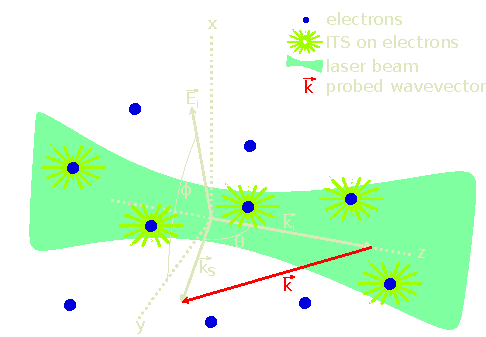
\includegraphics[width=0.2\paperwidth]{Scattering_Configuration_angles_bright.pdf}
    \end{column}
\end{columns}
        %the laser power: the length of the scattering volume: the wavelength width covered by each pixel of the detector, 
    With $c_{1}$ the total transmission factor obtained after a Raman calibration, $P_{i} L \delta \lambda$ some known experimental parameters,  $\frac{d \sigma_{T}}{d \Omega}(\theta, \phi)= r_{e}^{2}(1-sin^{2}\theta cos^{2} \phi)$ the differential Thomson scattering cross section along the observation direction and $I(\lambda)$ the normed instrument function. From a fitting of the scattered photons spectral intensity  the electron density ($n_{e}$) is directly obtained, $\Delta \lambda_{g}$ gives the electron temperature ($T_{e}$) and $\lambda_{0}-\lambda_{i}$ the electron drift velocity ($v_{e,drift}$).
    
    In case of Thomson signals with high signal to noise ratio, the Electron Energy Distribution Function (EEDF) can be extracted from the normed derivative of the spectral intensity$^{[2]}$: $f_{E}(E) \propto \frac{dI}{d\lambda}$ with $E=\frac{m_{e}}{2} \cdot \frac{c (\lambda-\lambda_{0})}{2 \lambda_{i} sin(\theta/2)}$.
 } 
%%%%%%%%%%%%%%%%%%%%%%%%%%%%%%%%%%%%%%%%%%%%%%%%%%%%%%%%%%%%%%%%%%%%%%%%%%%%%%%%%%%%%%%%%%%%%%%%%%% 
\end{tcbposter}


%%%%%%%%%%%%%%%%%%%%%%%%%%%%%%%%%%%%%%%%%%%%%%%%%%%%%%%%%%%%%%%%%%%%%%%%%%%%%%%%%%%%%%%%%%%%%%%%%%%
% Second (Experimental setup and results)
%%%%%%%%%%%%%%%%%%%%%%%%%%%%%%%%%%%%%%%%%%%%%%%%%%%%%%%%%%%%%%%%%%%%%%%%%%%%%%%%%%%%%%%%%%%%%%%%%%%

\vspace{.02\paperwidth}  

\begin{tcbposter}[
   poster = {columns=100,rows=2,colspacing=0mm , rowspacing=0.005\paperwidth , height=0.835\paperwidth , width=\paperwidth },
   no coverage ,
   boxes = {beamer,arc=10mm , colback=bleuet, colframe=bleuet, no shadow,, interior titled empty}	
   ]%,showframe} 
%%%%%%%%%%%%%%%%%%%%%%%%%%%%%%%%%%%%%%%%%%%%%%%%%%%%%%%%%%%%%%%%%%%%%%%%%%%%%%%%%%%%%%%%%%%%%%%%%%% 
  \posterbox[adjusted title= \color{beige} \faDotCircleO \ Experimental setup (THETIS$^{[3]}$) \faDotCircleO, sidebyside , righthand ratio=0.58, lower separated=false, sharp corners = southeast, sharp corners = southwest, ,natural height]{name=Exp,column=2,row=1,span=98}{ 
   \color{beige} 
   \small 
                \underline{Transmission branch:}
             \begin{itemize}
                 \item Q-switch Nd:YAG laser ($\lambda_{i}=532 \ nm$; $\tau=5 \ ns$;  $f=10 \ Hz$; $E=0.43 \ J$)
                 \item $2\ m$ focal lens $\Rightarrow$ laser beam waist $w_{0}\approx 0.3 \ mm$  %$\Rightarrow$ increase scattering intensity
                 \item Brewster windows, apertures and large aperture beam dump   $\Rightarrow$ reduce stray light propagation
             \end{itemize}

             \underline{Detection branch:}
             \begin{itemize}
                 \item Fiber bundle ($5 \times 3$, $0.3 \mu m$)  $\Rightarrow$ increase the etendue collected 
                 \item Volume Bragg Grating based Notch Filter (VBG-NF)  $\Rightarrow$ filter laser stray light contribution$^{[4]}$ with fewer losses than Triple Gratings Spectrometer (TGS)
                 \item Acton SP-2750 spectrometer  $\Rightarrow$ disperse the collected light
                 \item ICCD PI-MAX 5 camera (Gen II intensifier)  $\Rightarrow$ gated detection to reduce plasma stray light contribution and obtain temporal resolution
             \end{itemize} 

             \underline{Plasma sources under study:}
             
             \begin{itemize}
             \item Hall thruster and its electron source (thermo-emissive cathode)
             \item Planar magnetron (plasma assisted thin film deposition)
             \item ECR source (ion source for particle accelerators)
             \end{itemize}
             
\tcblower

    \vspace{-0.02\paperwidth}
             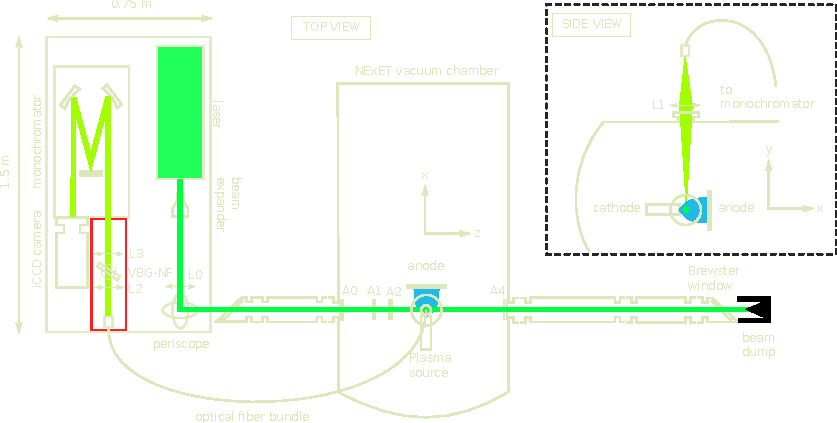
\includegraphics[width=0.545\paperwidth]{THETIS_on_NEXET_bright.pdf}             
   } 
%%%%%%%%%%%%%%%%%%%%%%%%%%%%%%%%%%%%%%%%%%%%%%%%%%%%%%%%%%%%%%%%%%%%%%%%%%%%%%%%%%%%%%%%%%%%%%%%%%%   
   \posterbox[adjusted title= \color{beige} \faDotCircleO \ Results \faDotCircleO, sidebyside, sidebyside align=top , righthand ratio=0.5, segmentation style={draw=verdatre,solid,line width= 4pt}, sharp corners = northeast, sharp corners = northwest]{name=Results,column=2,row=2,span=98,between=Exp and bottom}{ 
   \color{beige} 
   \small 
\underline{Cathode sources (spatial probing and EEDF):}

\begin{columns}  
   \begin{column}[T]{0.25\paperwidth}
   

   
\includegraphics[width=0.25\paperwidth]{Cathode_results/Thomson_spectra_fit_1p3mm_from_the_cathode_300mum.pdf}     
   
\includegraphics[width=0.25\paperwidth]{Cathode_results/EEDF_and_lnIntensity_vs_Energy.pdf}  

\includegraphics[width=0.25\paperwidth]{Cathode_results/Density_Temperature.pdf}   
 
   \end{column}
   
   \begin{column}[T]{0.22\paperwidth}
   \vspace{-0.034\paperwidth}%
   \includegraphics[width=0.22\paperwidth]{photos/Cathode_and_thruster} 
   
	\vspace{0.02\paperwidth}%
	  
   Thomson spectrum obtained $1.3 \ mm$ from the cathode orifice ($I_{discharge}=16 \ A $; $D_{Xe}=0.8 \ mg.s^{-1}$; $P_{chamber}=10^{-3} \ Pa$; $N_{averaged} = 6000 \ pulses $). %Savitzky–Golay filter for smoothing and derivative extraction.
   
   \vspace{0.04\paperwidth}%   
   
   EEDF extracted from the Thomson spectrum derivative.
   
     $\Rightarrow$ Weak deviations from ideal distribution coming from either the VBG-NF spectral distortion or Maxwell-Boltzmann distribution deviations (NB: the commonly used $ln(I_{T}) vs \Delta \lambda^{2}$ representation is not sensitive to such deviations).
   
\vspace{0.05\paperwidth}%   
   
$T_{e}$ and $n_{e}$ profiles obtained under the hypothesis of Maxwell-Boltzmann EVDF (i.e. Gaussian Thomson spectrum) for various discharge current and $D_{Xe} = 0.8 \ mg.s^{-1}$. 
   
   $\Rightarrow$ Expected increase of $T_{e}$ and $n_{e}$ with  discharge current. 
   
   $\Rightarrow$ Unexpected change of trend of $T_{e}$ at $ \approx 5 \ mm$ (visible for high discharge current).
   

   \end{column}
   
\end{columns}


   \tcblower
   \color{beige} 
   \small

   \underline{Magnetron source (spatio-temporal probing):}
   
\begin{columns}
   \begin{column}[T]{0.25\paperwidth}   
   
   \vspace{0.01\paperwidth}  
   
\includegraphics[width=0.25\paperwidth]{Magnetron_results/Density_Temperature.pdf}     
 
	\vspace{0.045\paperwidth}%   
 
\includegraphics[width=0.25\paperwidth]{Magnetron_results/Density_Temperature_velocity.pdf}     
    \end{column}
    
   \begin{column}[T]{0.22\paperwidth}

\vspace{0.0275\paperwidth}%   

   Temporal profile of $T_{e}$ and $n_{e}$ at $9 \ mm$ from the cathode of the magnetron, with a $10 \ Pa$ background pressure of Helium.
   
   $\Rightarrow$ Except during the unstable plasma ignition, precise temporal measurement of electron properties is achieved through synchronization of the discharge with the laser and $N_{avaeraged}= 6000 \ pulses$ .
   
   $\Rightarrow$ Steady $n_{e}$ ($\approx 5\times 10^{17} \ m^{-3}$) during the pulse and a linear increase of $T_{e}$ (up to $\approx 20 eV$). 
   
\vspace{0.06\paperwidth}%      
   
Axial profiles of $T_{e}$, $n_{e}$ and $v_{e,drift}$ obtained at $0 \ \mu s$ from the end of the pulse.

$\Rightarrow$ Monotonous decrease of  $T_{e}$ (possibly due to energy diffusion).

$\Rightarrow$ Non-monotonous behavior of  $n_{e}$ and $v_{e,drift}$ $\Rightarrow$ Possibly due to electric field inversion$^{[5]}$ and/or wave energization$^{[6]}$.  

   \vspace{0.046\paperwidth}%  
 %  \hspace*{0.005\paperwidth}
   \includegraphics[width=0.22\paperwidth]{photos/magnetron_LPGP2} 
  
  
   \end{column}
\end{columns}       
    
   }
   %%%%%%%%%%%%%%%%%%%%%%%%%%%%%%%%%%%%%%%%%%%%%%%%%%%%%%%%%%%%%%%%%%%%%%%%%%%%%%%%%%%%%%%%%%%%%%%%%%% 
   \end{tcbposter}  
   
     \vspace{0.02\paperwidth}  
\begin{tcbposter}[
   poster = {columns=100,rows=1,colspacing=0mm , width=\paperwidth},
   no coverage ,
   boxes = {beamer,arc=10mm,colback=bleuet, colframe=bleuet, no shadow, , interior titled empty}
   ]%showframe,
   
     \posterbox[adjusted title= \color{beige} \faDotCircleO \ Conclusion \faDotCircleO, ,natural height]{name=Conclu,column=2,row=1,span=98}{ 
   \color{beige} 
   \small
A new highly-sensitive ITS diagnostic has been successfully developed and applied  for electron property measurement in low-temperature plasmas. Electron properties measurements by ITS have been obtained for the first time in a Hall thruster cathode and a planar magnetron with spatial resolution of $ 0.3 \mu m$ and temporal resolution of $15 \ n s$.
   }
   
   \end{tcbposter}   
     
\end{frame}

\end{document}

